\documentclass[mathserif]{beamer}
\usetheme[secheader]{pecostalk}

\newcommand{\commentout}[1]{}

\newcommand{\cpp}[0]{\texttt{C++}}

\usepackage{accents}
\usepackage{amsfonts}
\usepackage{amsmath}
\usepackage{amssymb}
\usepackage{color}
\usepackage{mathtools}
\usepackage{subfigure}
\mathtoolsset{showonlyrefs,showmanualtags}

\definecolor{DarkGreen}{rgb}{0.13,0.55,0.13}

\graphicspath{{./figs/}}

\date{5-6 October 2010}
\author{Nathan V. Roberts}
\institute{Center for Predictive Engineering and Computational Sciences \\
  Institute for Computational Engineering and Sciences \\
  The University of Texas at Austin \\
  
  Joint work with \\
  Denis Ridzal, Pavel B. Bochev, Kara J. Peterson, Christopher M. Siefert at Sandia, and \\
  Leszek D. Demkowicz at UT Austin
}
\title[DPG: Stokes 2D]{
Application of a Discontinuous Petrov-Galerkin (DPG) Method to the Stokes Equations}
\begin{document}

\section{Introduction}

\begin{frame}
\titlepage
\end{frame}

\begin{frame}
\frametitle{Outline}
\tableofcontents
\end{frame}

\begin{frame}
\frametitle{Stokes Formulation}
\end{frame}

\frame{
%\begin{figure}[!htb]
%\center
%\includegraphics[scale=.28]{LDGcomparison.pdf}
%\caption{DPG with quasi-optimal test norm ($\beta=10^{-1}$) versus LDG convergence.}
%\end{figure}
}




\frame{
\frametitle{Experiments with parallel adaptivity}
We have implemented Heuer and Demkowicz's inner product in Camellia
\[
\left((\tau,v),(\delta \tau ,\delta v)\right)_V=C(K,\epsilon)\|v\| + \epsilon\| \nabla v\| + \|\beta \cdot \nabla v \|_w + \|\tau \|_w + \|\nabla \cdot \tau \|_w 
\]
where $C(K,\epsilon) = \min(\epsilon,|J(K)|)$. 
\begin{figure}[!h]
\centering
\subfigure{
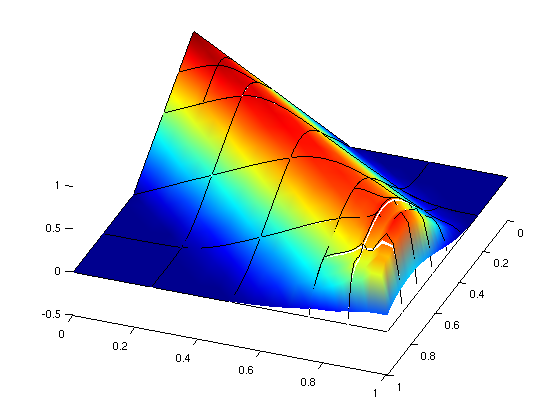
\includegraphics[scale=.3]{simplePlot.png}
}
\subfigure{
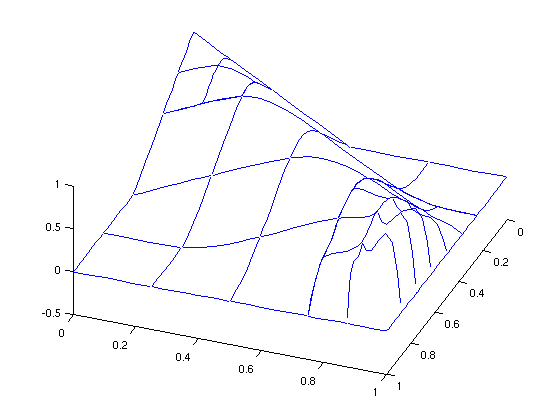
\includegraphics[scale=.3]{simpleFlux.png}
}
\end{figure}
}

\frame{
\frametitle{For better pictures, $\epsilon = 5e-2$.}

\begin{figure}[!h]
\centering
\subfigure{
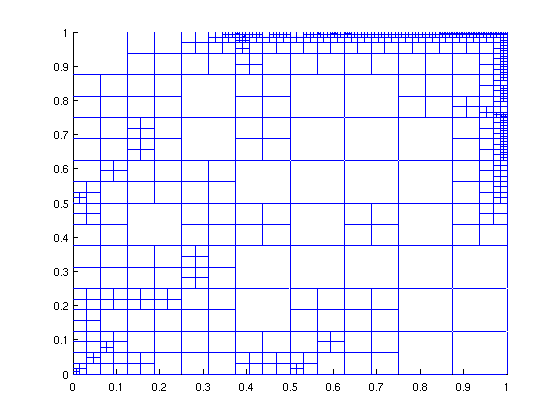
\includegraphics[scale=.25]{demoFlux.png}
}
\subfigure{
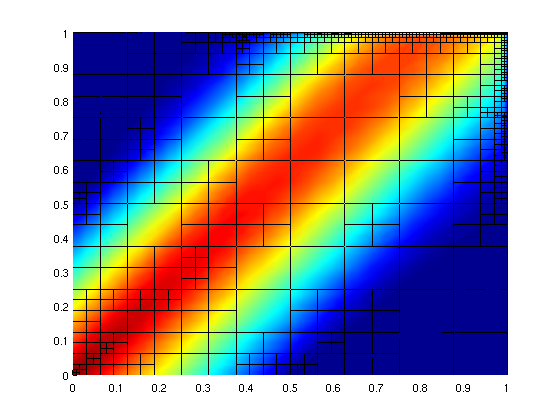
\includegraphics[scale=.25]{demoSolMesh.png}
}
\subfigure{
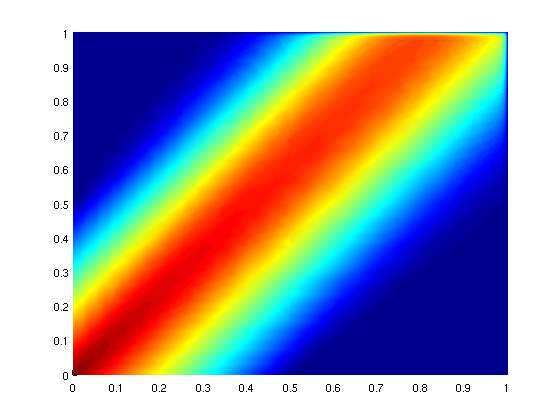
\includegraphics[scale=.25]{demoSol.png}
}
\end{figure}
}

\frame{
\frametitle{To make sure we still work at smaller scales, $\epsilon = 1e-3$}
\begin{figure}[!h]
\centering
\subfigure{
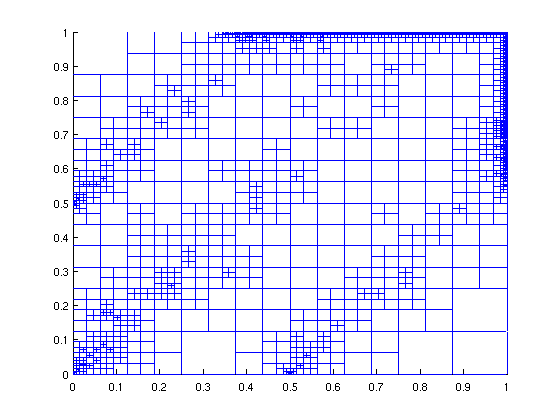
\includegraphics[scale=.35]{denseMesh.png}
}\subfigure{
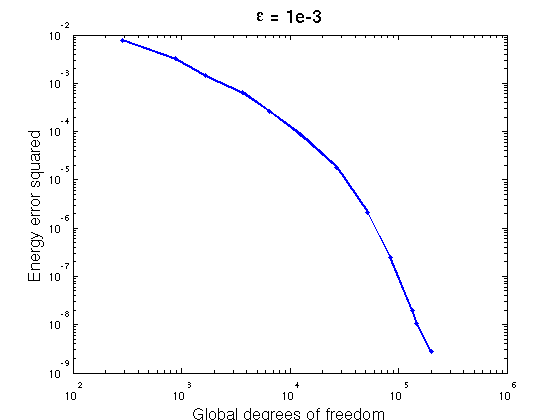
\includegraphics[scale=.35]{errorRate.png}
}
\end{figure}
}

\end{document}
